\section{eo\-Parse\-Tree\-Depth\-Init$<$ FType, Node $>$ Class Template Reference}
\label{classeo_parse_tree_depth_init}\index{eoParseTreeDepthInit@{eoParseTreeDepthInit}}
eo\-Parse\-Tree\-Depth\-Init : the initializer class for {\bf eo\-Parse\-Tree}{\rm (p.\,\pageref{classeo_parse_tree})}  


{\tt \#include $<$gp/eo\-Parse\-Tree\-Depth\-Init.h$>$}

Inheritance diagram for eo\-Parse\-Tree\-Depth\-Init$<$ FType, Node $>$::\begin{figure}[H]
\begin{center}
\leavevmode
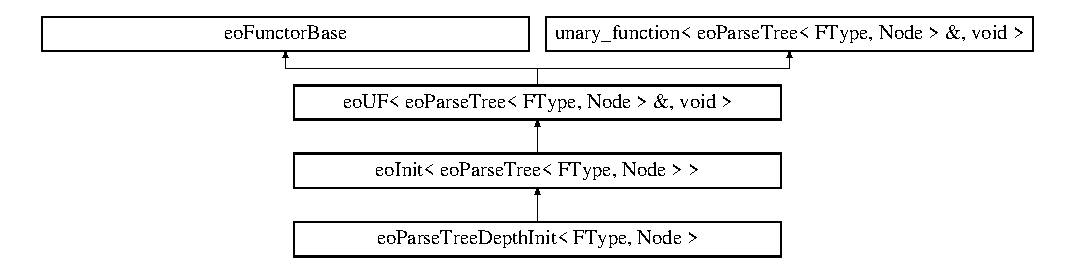
\includegraphics[height=3.21839cm]{classeo_parse_tree_depth_init}
\end{center}
\end{figure}
\subsection*{Public Types}
\begin{CompactItemize}
\item 
typedef {\bf eo\-Parse\-Tree}$<$ FType, Node $>$ {\bf Eo\-Type}\label{classeo_parse_tree_depth_init_w0}

\end{CompactItemize}
\subsection*{Public Member Functions}
\begin{CompactItemize}
\item 
{\bf eo\-Parse\-Tree\-Depth\-Init} (unsigned \_\-max\_\-depth, const std::vector$<$ Node $>$ \&\_\-initializor, bool \_\-grow=true, bool \_\-ramped\_\-half\_\-and\_\-half=false)
\begin{CompactList}\small\item\em Constructor. \item\end{CompactList}\item 
virtual std::string {\bf class\-Name} () const \label{classeo_parse_tree_depth_init_a1}

\begin{CompactList}\small\item\em My class name. \item\end{CompactList}\item 
void {\bf operator()} ({\bf Eo\-Type} \&\_\-tree)
\begin{CompactList}\small\item\em initialize a tree \item\end{CompactList}\end{CompactItemize}
\subsection*{Private Member Functions}
\begin{CompactItemize}
\item 
void {\bf generate} (std::list$<$ Node $>$ \&sequence, int the\_\-max, int last\_\-terminal=-1)\label{classeo_parse_tree_depth_init_d0}

\end{CompactItemize}
\subsection*{Private Attributes}
\begin{CompactItemize}
\item 
unsigned {\bf max\_\-depth}\label{classeo_parse_tree_depth_init_r0}

\item 
std::vector$<$ Node $>$ {\bf initializor}\label{classeo_parse_tree_depth_init_r1}

\item 
bool {\bf grow}\label{classeo_parse_tree_depth_init_r2}

\item 
bool {\bf ramped\_\-half\_\-and\_\-half}\label{classeo_parse_tree_depth_init_r3}

\item 
unsigned {\bf current\_\-depth}\label{classeo_parse_tree_depth_init_r4}

\end{CompactItemize}


\subsection{Detailed Description}
\subsubsection*{template$<$class FType, class Node$>$ class eo\-Parse\-Tree\-Depth\-Init$<$ FType, Node $>$}

eo\-Parse\-Tree\-Depth\-Init : the initializer class for {\bf eo\-Parse\-Tree}{\rm (p.\,\pageref{classeo_parse_tree})} 



Definition at line 48 of file eo\-Parse\-Tree\-Depth\-Init.h.

\subsection{Constructor \& Destructor Documentation}
\index{eoParseTreeDepthInit@{eo\-Parse\-Tree\-Depth\-Init}!eoParseTreeDepthInit@{eoParseTreeDepthInit}}
\index{eoParseTreeDepthInit@{eoParseTreeDepthInit}!eoParseTreeDepthInit@{eo\-Parse\-Tree\-Depth\-Init}}
\subsubsection{\setlength{\rightskip}{0pt plus 5cm}template$<$class FType, class Node$>$ {\bf eo\-Parse\-Tree\-Depth\-Init}$<$ FType, Node $>$::{\bf eo\-Parse\-Tree\-Depth\-Init} (unsigned {\em \_\-max\_\-depth}, const std::vector$<$ Node $>$ \& {\em \_\-initializor}, bool {\em \_\-grow} = {\tt true}, bool {\em \_\-ramped\_\-half\_\-and\_\-half} = {\tt false})\hspace{0.3cm}{\tt  [inline]}}\label{classeo_parse_tree_depth_init_a0}


Constructor. 

\_\-max\_\-depth The maximum depth of a tree \begin{Desc}
\item[Parameters:]
\begin{description}
\item[{\em \_\-initializor}]A std::vector containing the possible nodes \item[{\em \_\-grow}]False results in a full tree, True result is a randomly grown tree \item[{\em \_\-ramped\_\-half\_\-and\_\-half}]True results in Ramped Half and Half Initialization \end{description}
\end{Desc}


Definition at line 69 of file eo\-Parse\-Tree\-Depth\-Init.h.

\subsection{Member Function Documentation}
\index{eoParseTreeDepthInit@{eo\-Parse\-Tree\-Depth\-Init}!operator()@{operator()}}
\index{operator()@{operator()}!eoParseTreeDepthInit@{eo\-Parse\-Tree\-Depth\-Init}}
\subsubsection{\setlength{\rightskip}{0pt plus 5cm}template$<$class FType, class Node$>$ void {\bf eo\-Parse\-Tree\-Depth\-Init}$<$ FType, Node $>$::operator() ({\bf Eo\-Type} \& {\em \_\-tree})\hspace{0.3cm}{\tt  [inline]}}\label{classeo_parse_tree_depth_init_a2}


initialize a tree 

\begin{Desc}
\item[Parameters:]
\begin{description}
\item[{\em \_\-tree}]: the tree to be initialized \end{description}
\end{Desc}


Definition at line 96 of file eo\-Parse\-Tree\-Depth\-Init.h.

The documentation for this class was generated from the following file:\begin{CompactItemize}
\item 
eo\-Parse\-Tree\-Depth\-Init.h\end{CompactItemize}
